\chapter{Ergebnisse und Auswertung}
\label{ergebnisse}
\acresetall

In diesem Kapitel werden die Ergebnisse aller Tests vorgestellt und interpretiert.
Es werden zu jedem Test mögliche Erklärungen für dessen Ergebnis abgegeben.
Dabei wird in jedem Abschnitt eine der vier Forschungsfragen aus Kapitel~\ref{konzept} adressiert.

\section{Tempofehler}
{
	In diesem Abschnitt werden die Daten des Tests,
		die sich auf die Beantwortung der Frage~\ref{question:tempo} beziehen,
		dargestellt, ausgewertet und interpretiert.

	\subsection{Ergebnisse}
	{
		\begin{figure}[h]
			\hspace{-17mm}
			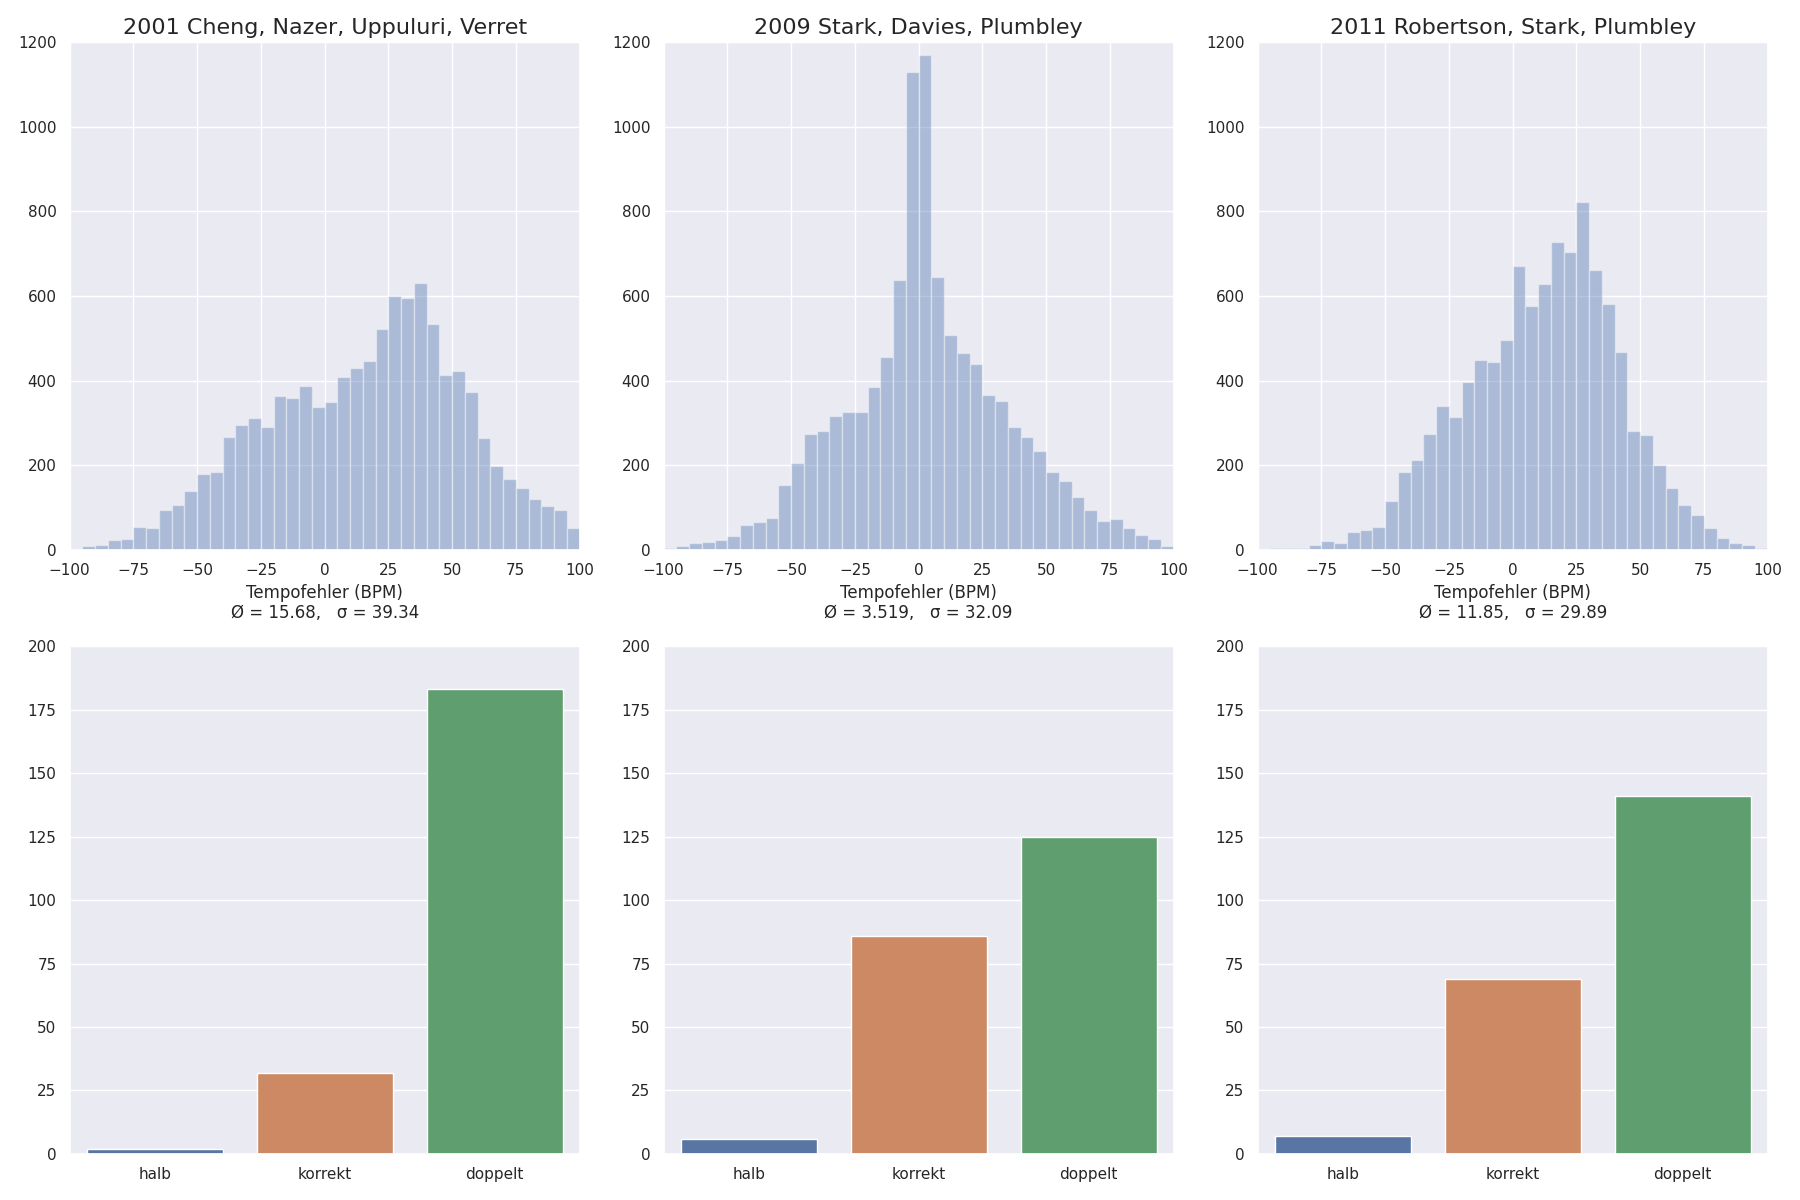
\includegraphics[scale=0.4]{resources/tempo_error_histogram.png}
			\caption{
				oben: Histogramme der Tempofehler, \\
				unten: Anzahl der Lieder, bei denen das halbe/korrekte/doppelte Tempo erkannt wurde
			}
			\label{fig:tempoerror}
		\end{figure}

		% Beschreibung Abbildung Tempofehler
		Die Histogramme in Abbildung~\ref{fig:tempoerror} zeigen die Verteilung der Tempofehler aller Lieder pro Algorithmus.
		Der abgebildete Bereich von \SI{-100}{\ac{BPM}} bis \SI{100}{\ac{BPM}} ist in \num{40} Balken unterteilt.
		So umfasst jeder Balken eine Spanne von \SI{5}{\ac{BPM}}.
		Die Balkendiagramme zeigen pro Algorithmus
			bei wie vielen Liedern das halbe, das korrekte oder das doppelte Tempo als Referenztempo genommen wurde.

	}

	\subsection{Auswertung}
	{
		% Auffälligkeiten der Abblidung
		Man kann deutlich erkennen,
			dass die Algorithmen von~\cite{2001_BeatThis} und~\cite{2011_PlRoSt} im Durchschnitt das Tempo etwas zu schnell schätzen.
		\cite{2009_DaPlSt} hingegen weicht im Durchschnitt nur minimal von einem Fehlerwert von 0 ab
			und erzielt Fehlerwerte,
			die sehr nah an 0 sind.
		Am meisten gestreut sind die Fehler bei \cite{2001_BeatThis}.
		Die Fehler von~\cite{2009_DaPlSt} haben eine etwas grö{\ss}ere Streuung (Standardabweichung) als die von~\cite{2011_PlRoSt}.
		Dennoch liefert~\cite{2009_DaPlSt} in diesem Vergleich die besten Tempovorhersagen,
			da dessen Durchschnittsfehlerwert am nähesten an \num{0} liegt.

		\begin{figure}[h]
			\centering
			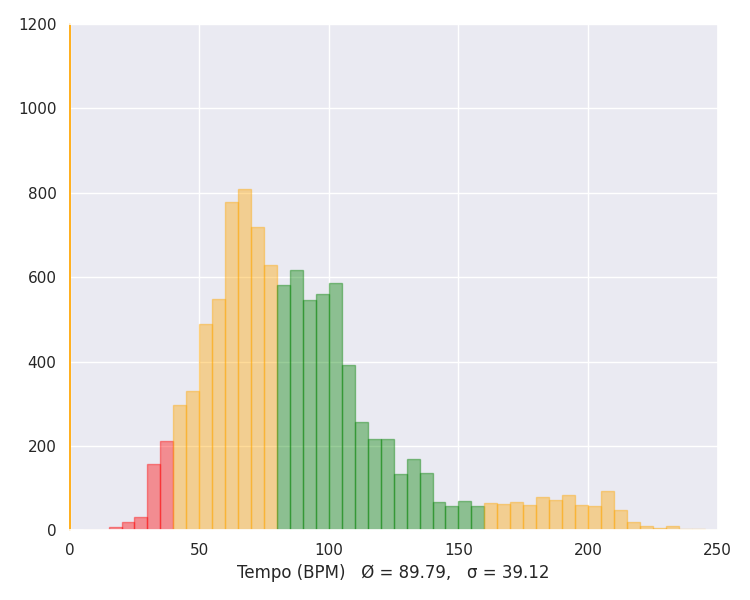
\includegraphics[scale=0.45]{resources/dataset_tempo_histogram.png}
			\caption{Tempoverteilung des Datensatzes}
			\label{fig:dataset_tempo}
		\end{figure}

		Zusätzlich ist anzumerken,
			dass bei jedem Algorithmus die meisten Lieder mit dem doppelten Tempo erkannt wurden.
		Dies resultiert hauptsächlich aus dem limitierten Ausgabebereich der Algorithmen von \SI{80}{\ac{BPM}} bis \SI{160}{\ac{BPM}}.
		Abbildung~\ref{fig:dataset_tempo} zeigt die Verteilung der Tempi aller Beatintervalle im Datensatz.
		Der grüne Bereich enthält \SI{44.44}{\percent} aller Beatintervalle
			und markiert den Tempobereich,
			den die Algorithmen direkt ausgeben können (\SI{80}{\ac{BPM}} bis \SI{160}{\ac{BPM}}).
		Der gelbe Bereich markiert den Tempobereich,
			den die Algorithmen mit Berücksichtigung von Halb- und Doppeltempofehlern ausgeben können.
		Dieser Bereich erstreckt sich von \SI{40}{\ac{BPM}} bis \SI{80}{\ac{BPM}} und von \SI{160}{\ac{BPM}} bis \SI{320}{\ac{BPM}}
			und enthält \SI{51.45}{\percent} aller Beatintervalle,
			wobei sich die meisten davon im untern Tempobereich befinden.
		Dies erklärt,
			warum so viele Lieder mit doppeltem Tempo erkannt wurden.
		Der rote Bereich umfasst alles au{\ss}erhalb von \SI{40}{\ac{BPM}} bis \SI{320}{\ac{BPM}}
			und markiert den Tempobereich,
			den die Algorithmen unmöglich bestimmen können.
		Dieser Bereich enthält \SI{4.11}{\percent} aller Beatintervalle.

		% Mögliche Erklärung 1 (ODF)
		Ein möglicher Grund für die ungenauen Tempovorhersagen des Algorithmus von~\cite{2001_BeatThis}
			ist,
			dass dieser eine einfachere \ac{ODF} verwendet.
		Die \ac{ODF} basiert auf einer Glättung und einer anschlie{\ss}enden Differentiation.
		So werden nur schnelle Anstiege der Lautstärke extrahiert,
			während bei der \ac{ODF} der anderen beiden Algorithmen auch die Änderungen der Phase im Signal berücksichtigt
			und so auch Tonänderungen,
			bei denen die Lautstärke gleichbleibt,
			als Einsätze erkannt werden.

		% Mögliche Erklärung 2 (Tempo Induction)
		Au{\ss}erdem verwendet~\cite{2001_BeatThis} zur Tempobestimmung Kammfilter mit drei Zähnen,
			welche einen ähnlichen Effekt haben wie eine \ac{ACF}.
		Bei der \ac{ACF} wird das Signal mit einer verzögerten Version von sich selbst elementweise multipliziert.
		Bei diesem Kammfilter wird das Signal mit zwei verzögerten Versionen von sich selbst elementweise addiert.
		Beide Operationen haben den Effekt,
			dass sich bei der richtigen Verzögerung
			die regelmä{\ss}igen Peaks des Signals überlagern
			und so die Ausgabe einen gro{\ss}en Wert annimmt.
		Ein Signal,
			was sich beispielsweise alle $T$ Sekunden wiederholt,
			wiederholt sich gleichzeitig auch alle $2T, 3T,$ usw. Sekunden.
		Dadurch entstehen in der \ac{ACF} sowie in der Kammfilterausgabe mehrere Peaks jeweils bei Vielfachen des ersten Peaks.
		\cite{2001_BeatThis} hört an dieser Stelle auf
			und bestimmt den grö{\ss}ten Peak als Beatperiode des Songs,
			während die anderen Peaks ignoriert werden.
		\cite{2009_DaPlSt} hingegen multipliziert anschlie{\ss}end die Ausgabe der \ac{ACF} mit mehreren Kammfiltern,
			um die Abstände von äquidistanten Peaks in der \ac{ACF} zu ermitteln.

		% 2009 vs. 2011 (vorverarbeitete ODF)
		Die Tempobestimmung von~\cite{2011_PlRoSt} lässt sich schwierig mit der der anderen beiden Algorithmen vergleichen,
			da sie auf einem komplett anderen Prinzip beruht.
		Es lässt sich aber in der Visualisierung der Algorithmen erkennen,
			dass die vorverarbeitete \ac{ODF} von~\cite{2009_DaPlSt} deutlichere und prägnantere Peaks aufweist
			als die von~\cite{2011_PlRoSt}.
		Anhand dessen lassen sich die unterschiedlichen Ergebnisse dieser beiden Algorithmen teilweise erklären.

		% 2009 vs. 2011 (Einlaufzeit)
		Eine weitere Erklärung für die schlechteren Ergebnisse von~\cite{2011_PlRoSt} könnte sein,
			dass dessen Algorithmus mehr Zeit benötigt,
			um das richtige Tempo zu finden.
		Dadurch könnten am Anfang des Songs viele Tempovorhersagen ungenau sein.
	}
}

\section{Beatzeitpunktfehler}
{
	\label{ergebnisse/beatzeitpunktfehler}

	In diesem Abschnitt werden die Daten des Tests,
		die sich auf die Beantwortung der Frage~\ref{question:beat} beziehen,
		dargestellt, ausgewertet und interpretiert.

	\subsection{Ergebnisse}
	{
		\begin{figure}[h]
			\centering
			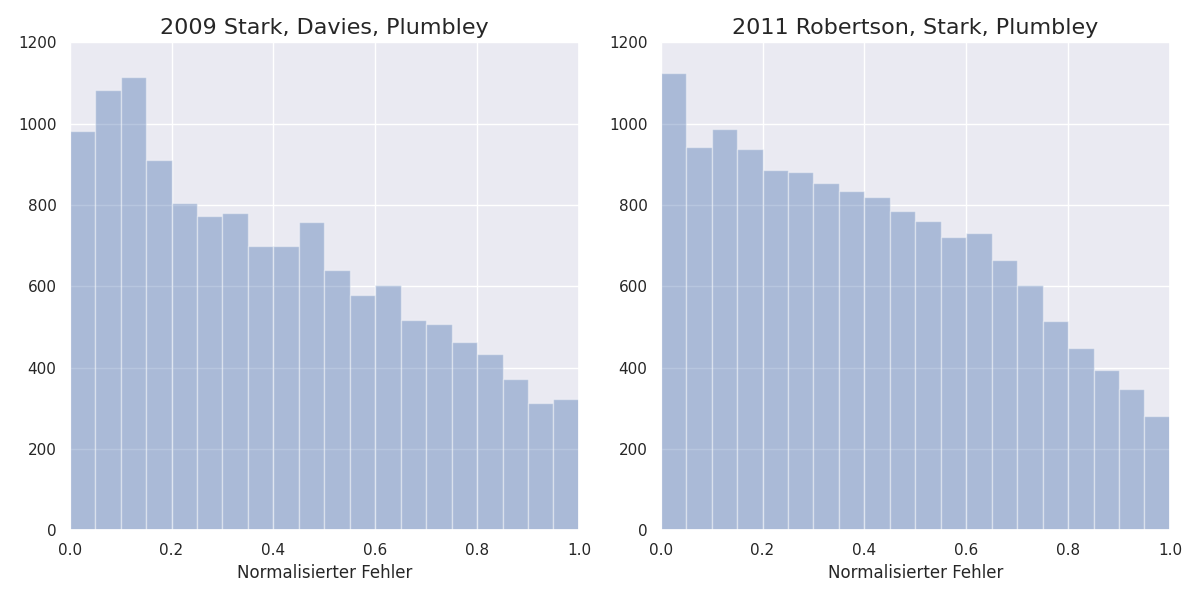
\includegraphics[scale=0.47]{resources/beat_positions.png}
			\caption{Histogramme der Beatzeitpunktfehler}
			\label{fig:beaterror}
		\end{figure}

		\begin{table}[h]
			\centering
			\begin{tabular}{l | r | r}
				                            & \cite{2009_DaPlSt} & \cite{2011_PlRoSt} \\
				\hline \hline
				Anzahl korrekter Beats      & \num{14944}        & \num{15951}        \\
				davon ungepaart             &  \num{1600}        &  \num{1437}        \\
				\hline
				Anzahl vorhergesagter Beats & \num{16361}        & \num{24426}        \\
				davon ungepaart             &  \num{3017}        &  \num{9912}        \\
				\hline
				Anzahl der Beatpaare        & \num{13344}        & \num{14514}
			\end{tabular}
			\caption{Anzahl korrekter und vorhergesagter Beats}
			\label{tab:pairnum}
		\end{table}

		In Abbildung~\ref{fig:beaterror} ist die Verteilung der Fehler aller Beatpaare zu sehen.
		Die Histogramme zeigen nur die Fehler der gepaarten Beats,
			enthalten jedoch keine Informationen über die ungepaarten Beatvorhersagen.
		Wie viele der korrekten und vorhergesagten Beats gepaart wurden,
			kann aus Tabelle~\ref{tab:pairnum} entnommen werden.
		Die unterschiedlichen Zahlen für die Anzahl korrekter Beats kommen daher,
			dass die Lieder
			(je nachdem ob sie der Algorithmus mit halbem, korrektem oder doppeltem Tempo erkennt)
			unterschiedlich viele Beats haben.
	}

	\subsection{Auswertung}
	{
		% Histogramauswertung
		In den beiden Histogrammen kann erkannt werden,
			dass beide Algorithmen eine ähnliche Fehlerverteilung haben,
			welche auch zeigt,
			dass es mehr Beatvorhersagen in der Nähe der korrekten Beats gibt.
		Diese Information bezieht sich jedoch nur auf die gepaarten Schläge.
		Aus Tabelle~\ref{tab:pairnum} kann abgelesen werden,
			dass zwar beide Algorithmen ungefähr gleich viele Beatvorhersagen hätten machen müssen (Anzahl korrekter Beats),
			aber~\cite{2011_PlRoSt} viel mehr Beatzeitpunkte ausgegeben hat (Anzahl vorhergesagter Beats).
		Dies hatte zu Folge,
			dass es öfter dazu kam,
			dass mehrere vorhergesagte Beats in die Nähe eines korrekten Beats fielen
			und somit mehr ungepaarte Beats generiert wurden.
		Das bedeutet,
			dass die Beatvorhersagen von beiden Algorithmen ungefähr die gleiche Genauigkeit haben,
			aber~\cite{2011_PlRoSt} zu viele Beats ausgibt.

		% Erklärung
		Eine mögliche Erklärung dafür ist,
			dass \cite{2011_PlRoSt} das Tempo zu schnell schätzt,
			was durch Abbildung~\ref{fig:tempoerror} bestätigt wird.
		Dadurch werden mehr Schläge pro Minute ausgegeben.
		Oft bleibt der Algorithmus auch auf einer Tempo-Phase-Hypothese hängen.
		Wenn diese weit genug weg von den tatsächlichen Werten von Tempo und Phase entfernt ist,
			bewirkt die Tempoupdateregel ---
			deren eigentlicher Zweck es ist,
			dass die Tempo-Phase-Hypothese nicht zu schnell zu weit springen kann ---
			dass sich die Ausgabe von Tempo und Phase überhaupt nicht ändert.
	}
}

\section{längste korrekte Beatfolge}
{
	In diesem Abschnitt werden die Daten des Tests,
		die sich auf die Beantwortung der Frage~\ref{question:streak} beziehen,
 		dargestellt, ausgewertet und interpretiert

	\subsection{Ergebnisse}
	{
		\begin{figure}[h]
			\centering
			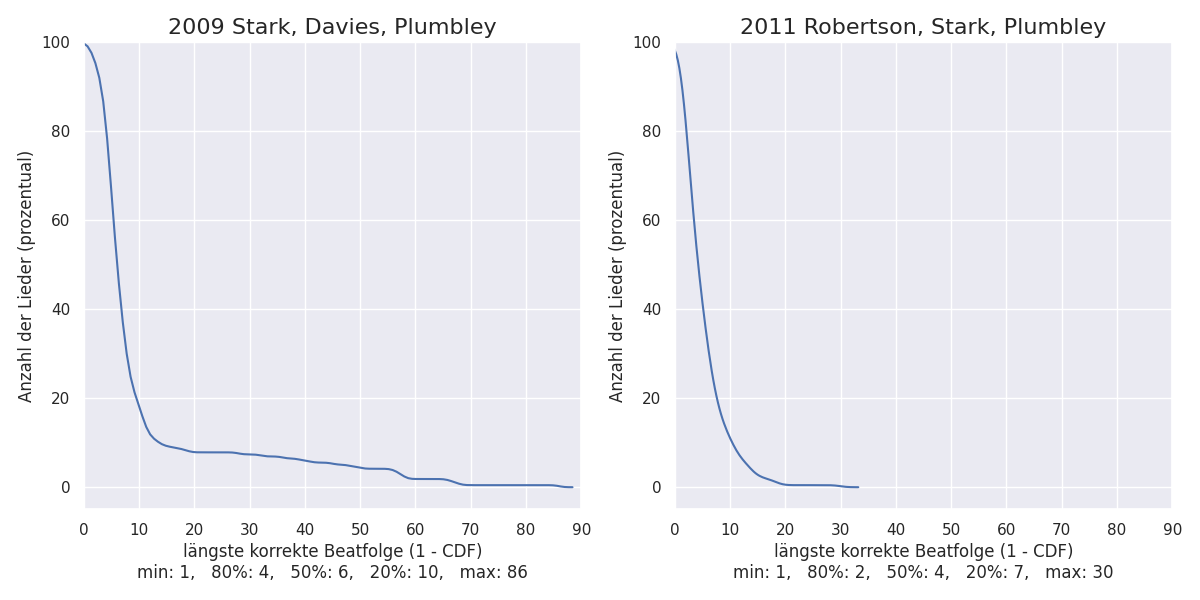
\includegraphics[scale=0.47]{resources/longest_streak.png}
			\caption{Verteilung der längsten korrekten Beatfolgen}
			\label{fig:longest_streak}
		\end{figure}

		Die Graphen in Abbildung~\ref{fig:longest_streak} zeigen eine vertikal gespiegelte kumulative Verteilungsfunktion.
		So kann man für jede Beatfolgenlänge ablsesen,
			in wie vielen Liedern (prozentual) eine korrekte Beatfolge mit mindestens dieser Länge erkannt wurde.

		Die längste korrekte Beatfolge von~\cite{2009_DaPlSt} ist \num{86}.
		\cite{2011_PlRoSt} hingegen erfasste eine maximale Beatfolge von \num{30} Schlägen korrekt.
		Generell hat~\cite{2009_DaPlSt} für jede beliebige Beatfolgenlänge eine grö{\ss}ere Anzahl an Liedern,
			bei denen eine mindestens so lange Beatfolge korrekt erfasst wurde.
	}

	\subsection{Auswertung}
	{
		Die Ergebnisse hier lassen sich genauso wie die Ergebnisse in Abschnitt~\ref{ergebnisse/beatzeitpunktfehler} erklären.
		\cite{2011_PlRoSt} hat das Tempo zu schnell geschätzt,
			wodurch zu viele Beatzeitpunkte ausgegeben wurden.
		Dadurch wird jede lange korrekte Beatfolge durch viele ungepaarte Beats unterbrochen.
	}

}

\section{Rechenzeit}
{
	In diesem Abschnitt werden die Daten des Tests,
		die sich auf die Beantwortung der Frage~\ref{question:cpu_time} beziehen,
 		dargestellt, ausgewertet und interpretiert.

	\subsection{Ergebnisse}
	{
		\begin{table}[h]
			\centering
			\begin{tabular}{l | r | r | r}
				                       & \cite{2001_BeatThis} & \cite{2009_DaPlSt}   & \cite{2011_PlRoSt} \\
				\hline \hline
				Gesamtrechenzeit       & \SI{979.1}{\second}  & \SI{352.2}{\second} & \SI{2796}{\second} \\
				pro Sekunde Audioinput & \SI{112.8}{\milli\second} & \SI{40.58}{\milli\second} & \SI{322.1}{\milli\second}
			\end{tabular}
			\caption{Rechenzeiten der Algorithmen}
			\label{tab:cputime}
		\end{table}

		Tabelle~\ref{tab:cputime} zeigt die Gesamtrechenzeiten,
			die jeder Algorithmus für die Verarbeitung aller Lieder im Datensatz gebraucht hat,
			sowie die benötigte Rechenzeit pro Sekunde Audioeingabe.
		Damit ist die Zeit gemeint,
			die im Durchschnitt benötigt,
			wird um \num{44100} Audiosamples zu verarbeiten.
		Die Gesamtlänge aller Lieder im Datensatz beträgt \SI{8680}{\second}.
	}

	\subsection{Auswertung}
	{
		% Who wins?
		Da alle Algorithmen auf derselben Hardware getestet wurden,
			lassen sich die gemessenen Zeiten untereinander vergleichen.
		Somit geht~\cite{2009_DaPlSt} aus diesem Tests als klarer Sieger hervor,
			gefolgt von~\cite{2001_BeatThis} und zuletzt~\cite{2011_PlRoSt}.

		% Erklärung
		Die Unterschiede in der Rechenzeit lassen sich zum einen auf die unterschiedlichen Aktualisierungsraten der Tempovorhersagen
			und zum anderen auf die unterschiedlichen Datenmengen,
			die die Algorithmen verarbeiten,
			zurückführen.
		% Updatezeiten
		Während~\cite{2009_DaPlSt} die Tempoberechnung alle \SI{1.5}{\second} durchführt,
			aktualisiert die für diese Arbeit angefertigte Implementierung von~\cite{2001_BeatThis} die Tempovorhersage jede Sekunde
			und~\cite{2011_PlRoSt} alle \SI{11.61}{\milli\second}.
		% Datenmengen
		Au{\ss}erdem arbeitet \cite{2001_BeatThis} direkt auf Audiosamples
			mit einer Abtastfrequenz von \SI{44.1}{\kilo\hertz}
			statt auf einer \ac{ODF} mit einer Abtastfrequenz von $1 / \SI{11.61}{\milli\second} = \SI{86}{\hertz}$.
		Dadurch ist der \SI{1.09}{\second} lange Analyserahmen schon $\SI{1.09}{\second} \cdot \SI{44.1}{\kilo\hertz} \cdot \SI{4}{\byte} = \SI{187}{\kibi\byte}$ lang (\num{4} Byte pro Sample, da das Single-Precision-Gleitkommaformat aus dem \acs{IEEE} 754 Standard verwendet wurde).
		Dazu kommt,
			dass~\cite{2001_BeatThis} zweimal eine \ac{FFT} und eine \ac{IFFT} mit einer Zeitkomplexität von $O(n\log(n))$ auf diesem Array berechnet,
			während~\cite{2009_DaPlSt} fast nur Operationen mit linearer Zeitkomplexität ausführt.
		Die anderen beiden Algorithmen berechnen zwar auch eine \ac{STFT} (wiederholte \ac{FFT}) auf dem Eingangssignal,
			jedoch nur auf jeweils \num{512} Samples gro{\ss}en Arrays (\SI{2}{\kibi\byte})
		Der Analyserahmen von~\cite{2009_DaPlSt} umfasst zwar \SI{6}{\second},
			ist aber nur \num{512} Samples lang,
			da es sich um \ac{ODF}-Samples handelt.
		Dadurch werden in jedem Verarbeitungsschritt viel kleinere Datenmengen verarbeitet.
		Auch die Kammfiltermatrix aus~\cite{2011_PlRoSt} basiert auf \ac{ODF}-Samples
			und besteht deshalb aus $32 + 33 + ... + 65 = 1649$ Samples.
		Diese wird pro Temposchätzung zwei Mal komplett durchlaufen.

		Zusammenfassend lässt sich sagen,
			dass \cite{2011_PlRoSt} wenig Daten verarbeitet.
			jedoch mit einer hohen Aktualisierungsrate arbeitet,
			wodurch der gro{\ss}e Rechenaufwand zustande kommt.
		\cite{2001_BeatThis} verarbeitet viele Daten,
			jedoch mit einer geringen Aktualisierungsrate,
			wodurch ebenfalls ein gro{\ss}er Rechenaufwand zustande kommt.
		\cite{2009_DaPlSt} verarbeitet kleine Datenmengen kombiniert mit einer geringen Aktualisierungsrate,
			wodurch der geringe Rechenaufwand zustande kommt.

		Abschlie{\ss}end lässt sich anmerken,
			dass die gemessenen Zeiten implementierungsabhängig sind.
		Das Aktualisierungsintervall von einer Sekunde bei~\cite{2001_BeatThis} ist beispielsweise willkürlich gewählt.
		Die ausschlaggebenden Faktoren,
			mit denen die unterschiedlichen Rechenzeiten erklärt wurden
			(Grö{\ss}e der Analyserahmen, Updateintervall des 2009er und 2011er Algorithmus, etc.),
			kommen von den Algorithmenbeschreibungen der ursprünglichen Paper
			und sind nicht der Implementierung zu verschulden.
	}
}
